% !TEX options=--shell-escape
% Beamer template by Julian Lueken

\documentclass[8pt, aspectratio=169]{beamer}
\usepackage[main=ngerman]{babel}
\usepackage[T1]{fontenc}
\usepackage{tikz}
\usepackage{helvet}
\usepackage{lipsum}
\usepackage{float}
\usepackage{svg}
\usepackage{subcaption}
\usepackage{pifont}
\renewcommand{\familydefault}{\sfdefault}


% set theme color to DLR logo color
\definecolor{mypres}{RGB}{97,107,104}

% set presentation date
\day30\relax
\month01\relax
\year2023\relax

% set big cdot for header
\makeatletter
\newcommand*\bigcdot{\mathpalette\bigcdot@{.5}}
\newcommand*\bigcdot@[2]{\mathbin{\vcenter{\hbox{\scalebox{#2}{$\m@th#1\bullet$}}}}}
\makeatother

% setting some colors for the theme
\setbeamercolor{palette primary}{fg=mypres,bg=white}
\setbeamercolor{palette secondary}{fg=mypres,bg=white}
\setbeamercolor{structure}{fg=mypres,bg=white}
\setbeamercolor{title in head/foot}{fg=black,bg=white}
\setbeamercolor{date in head/foot}{fg=gray,bg=white}

% definition of the headline template
\defbeamertemplate*{headline}{mytheme}{%
	\begin{tikzpicture}[remember picture, overlay]
		\node[text=mypres,anchor=west,font=\sffamily\tiny,text width=0.8\paperwidth] at ([xshift=7pt,yshift=0.5\textheight]current page.west) (header0) {DLR.de{ }$\bigcdot${ }Folie \insertframenumber};
		\node[text=mypres,anchor=west,font=\sffamily\tiny,text width=0.8\paperwidth] at ([xshift=55pt,yshift=0.5\textheight]current page.west) (header1) {$\bigcdot${ }\insertshorttitle{ }$\bigcdot${ }\insertauthor{ }$\bigcdot${ }\insertdate};
	\end{tikzpicture}
	\vskip15pt
}

% definition of the footline template arial
\defbeamertemplate*{footline}{mytheme}{%
	\begin{tikzpicture}[remember picture, overlay]
		\node[inner sep=0, anchor = south east] at (current page.south east) (banner) {
\includegraphics[page=1, width=\paperwidth]{footer.pdf}};
	\end{tikzpicture}
	\vskip0pt
}

% definition of the title page template
\defbeamertemplate*{title page}{mytheme}[1][] {
	\begin{tikzpicture}[remember picture, overlay]
		\node[text=mypres,anchor=west,font=\sffamily\tiny,text width=0.8\paperwidth] at ([xshift=6pt,yshift=0.5\textheight]current page.west) (header0) {DLR.de{ }$\bigcdot${ }Folie \insertframenumber};
		\node[text=mypres,anchor=west,font=\sffamily\tiny,text width=0.8\paperwidth] at ([xshift=54pt,yshift=0.5\textheight]current page.west) (header1) {$\bigcdot${ }\insertshorttitle{ }$\bigcdot${ }\insertauthor{ }$\bigcdot${ }\insertdate};
		\node[inner sep=0, anchor = south east] at (current page.south east) (banner) {
\includegraphics[page=1, width=\paperwidth]{header.pdf}};
		\node[text=mypres,anchor=south west,font=\sffamily\LARGE,text width=0.8\paperwidth] at ([xshift=7pt,yshift=1.50cm]current page.west) (title) {\raggedleft\insertshorttitle};
		\node[text=mypres,anchor=south west,font=\sffamily\large,text width=0.8\paperwidth] at ([xshift=7pt,yshift=1.00cm]current page.west) (subtitle) {\raggedleft\inserttitle};
		\node[text=mypres,anchor=south west,font=\sffamily,text width=.55\paperwidth] at ([xshift=7pt,yshift=-1cm]current page.west) (author) {\raggedright\insertauthor};
		\node[text=mypres,anchor=south west,font=\sffamily,text width=.55\paperwidth] at ([xshift=7pt,yshift=-1.5cm]current page.west) (date) {\raggedright\insertdate};
	\end{tikzpicture}
	\vskip0pt
}

% remove navigation symbols
\setbeamertemplate{navigation symbols}{}

\title[CoolingGen]{Eine Software zur Erstellung von Kühlungsgeometrien}
\author{Julian Lüken}
\date{\today}

\begin{document}

\begin{frame}[plain]
	\maketitle
\end{frame}

\begin{frame}
	\frametitle{Problemstellung / Kühlung}
	\vspace{-1cm}\hspace{-0.5cm}
	\centering
	\begin{minipage}[t]{0.8\textwidth}
		\centering
		\hspace{0.36\textwidth}
		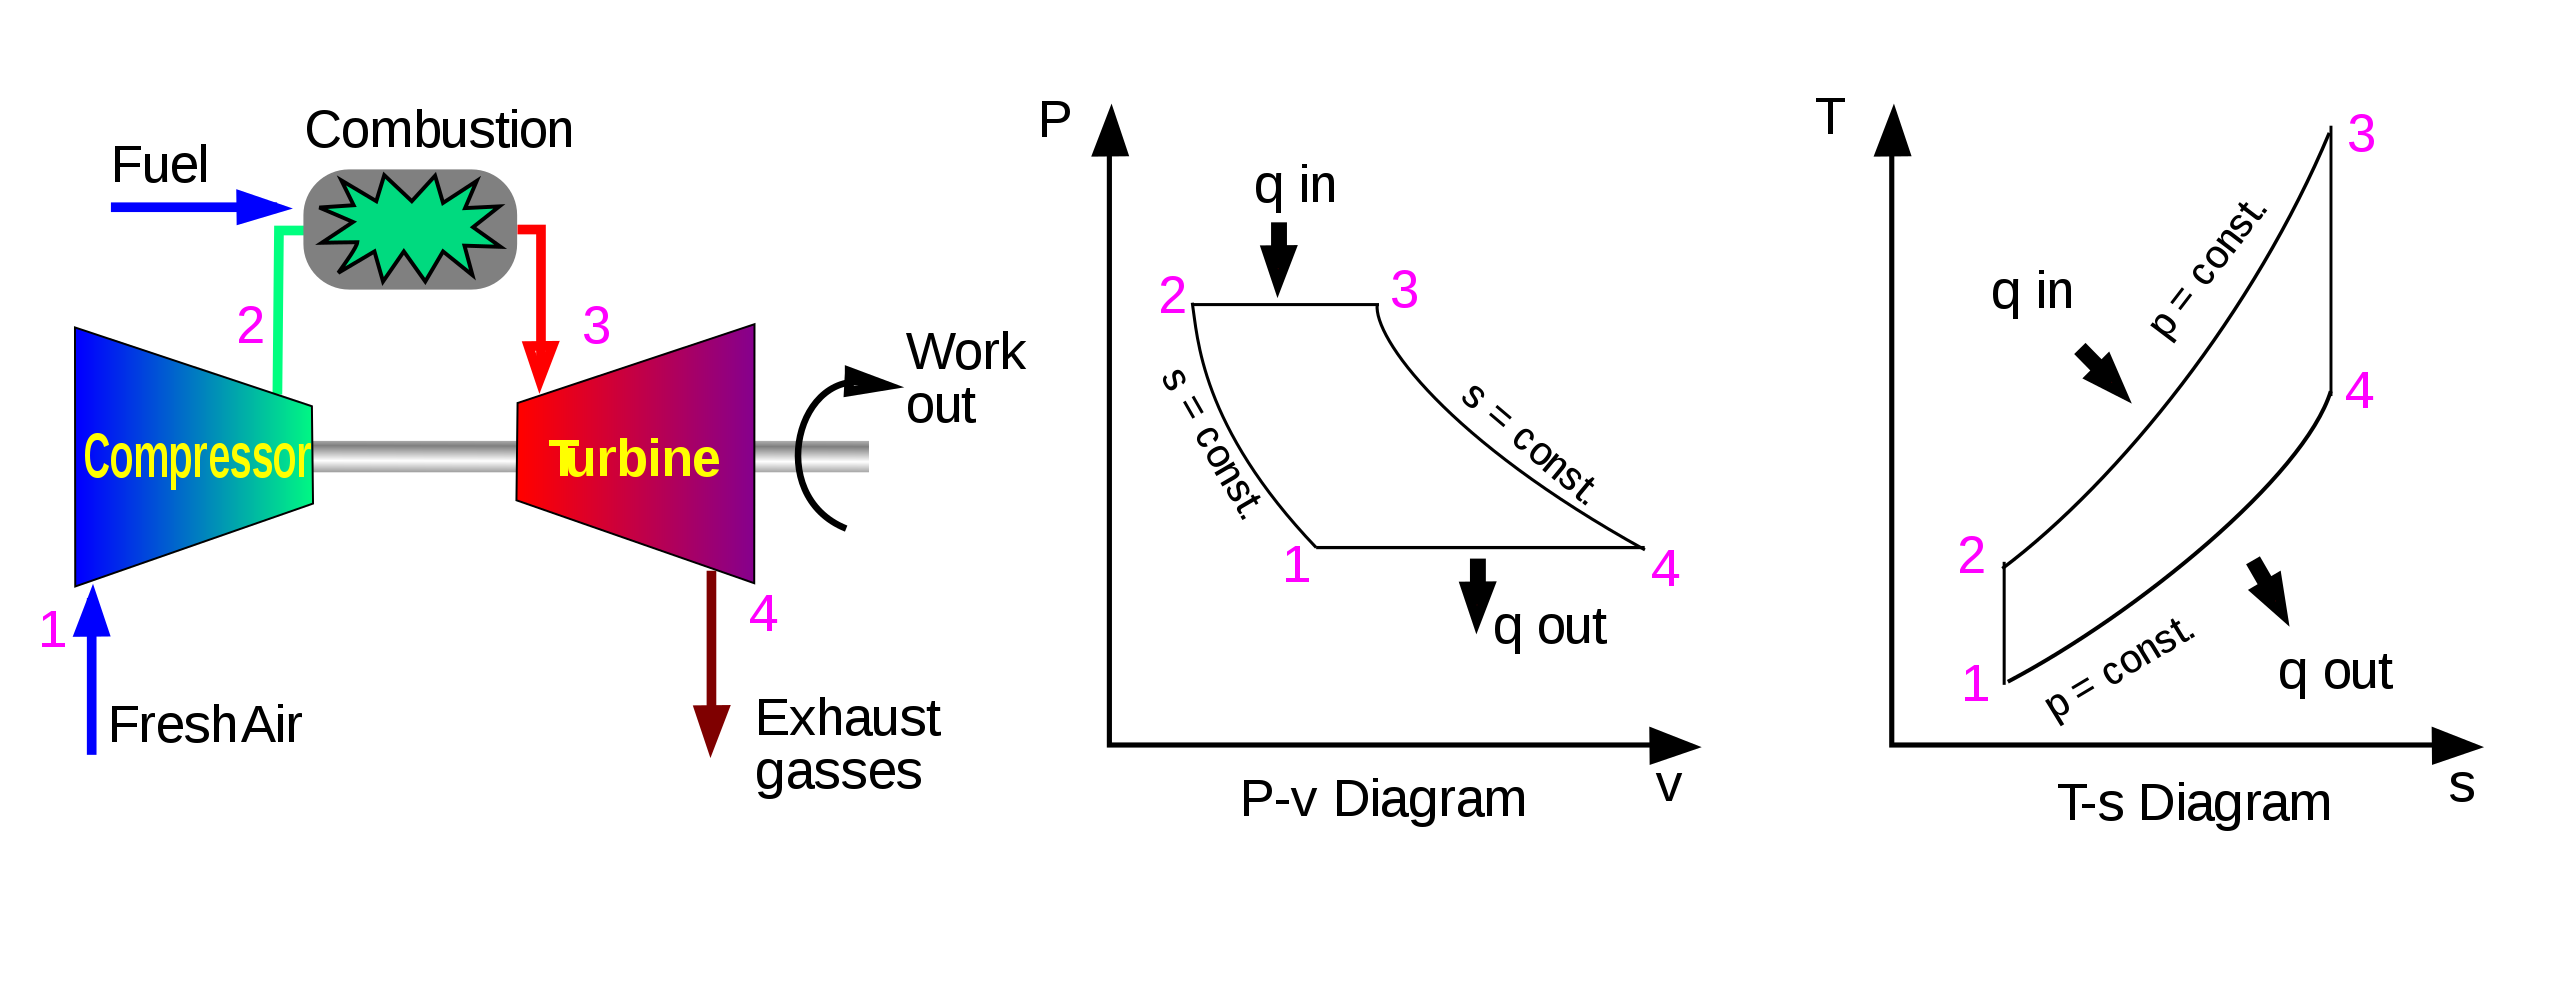
\includegraphics[width=0.625\textwidth]{images/Brayton_cycle.svg.png}
	\end{minipage}
	\begin{minipage}[t]{\textwidth}
		\begin{itemize}
			\item Effizienz der Turbine kann theoretisch durch großen Temperaturgradienten erhöht werden
			\item[] 	\textrightarrow{} Praktisch strebt man darum hohe Temperaturen in der Brennkammer an
			\item 		\textbf{Aber:} Hohe thermische Last der Turbinenschaufeln führt zu starker Abnutzung
			\item[] 	\textrightarrow{} Kühlung wird benötigt
			\item 		\textbf{Aber:} Die Kühlung wiederum nutzt Luftstrom, der nicht für den Antrieb benutzt werden kann
			\item[] 	\textrightarrow{} Negativer Einfluss auf Wirkungsgrad
			\item[] 	{}
			\item[\textrightarrow] Wir folgern: \textbf{Kühlungsdesign ist Filigranarbeit!}
		\end{itemize}
	\end{minipage}
	\vfill
\end{frame}

\begin{frame}
	\frametitle{Problemstellung / Kühlung}
	\vspace{-1cm}\hspace{-0.5cm}
	\begin{minipage}[t]{0.5\textwidth}
		Kühlungsdesign setzt sich u.a. aus den folgenden Aspekten zusammen:
		\begin{itemize}
			\item Auswahl/Konditionierung der Kühlluft
			\item Auswahl der verwendeten Werkstoffe
			\item \textbf{Gestaltung der Kühlstrukturen}
		\end{itemize}
		\vspace{1em}
		Diese \textbf{Kühlstrukturen} beinhalten
		\begin{itemize}
			\item \textbf{Kühlkanäle} ("cooling channels"),
			\item \textbf{Prallkühlung} ("{}impingement cooling"),
			\item Rippen ("rib turbulators"),
			\item \textbf{Filmkühlung} ("film cooling"),
			\item \textbf{Pin-fins},
			\item und \textbf{Ausblasungsschlitze} ("trailing edge slots").
		\end{itemize}
	\end{minipage}
	\begin{minipage}[t]{0.48\textwidth}
			\begin{figure}[H]
			\centering
			\begin{subfigure}{.49\textwidth}
				\centering
				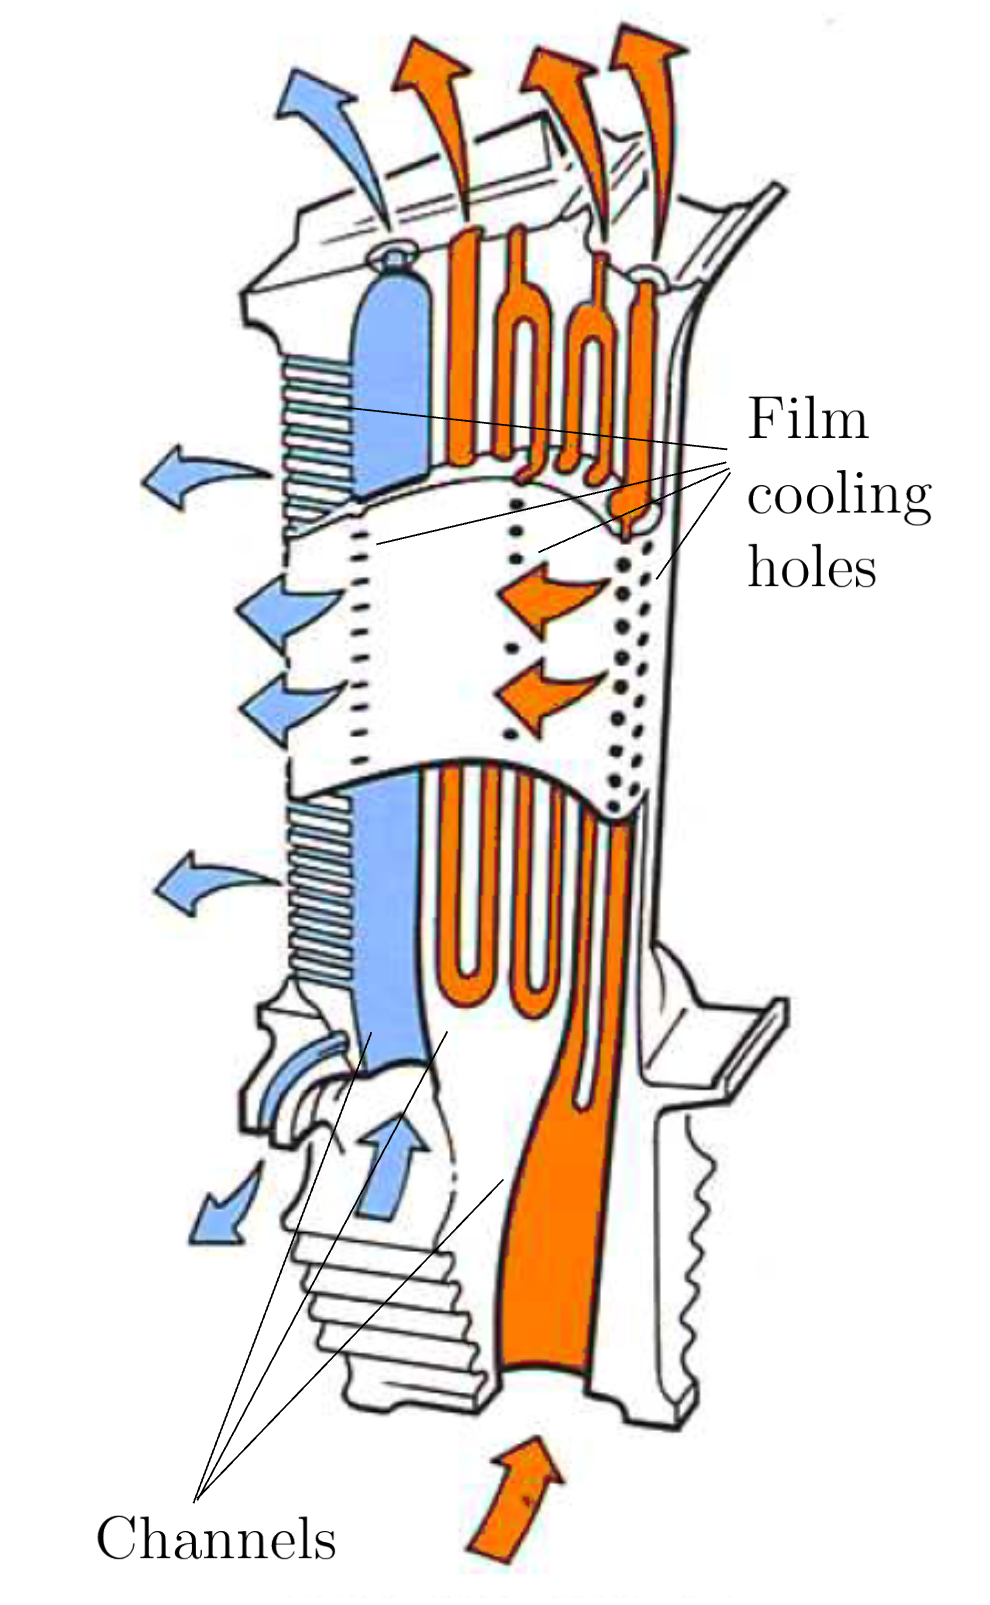
\includegraphics[width=.8\textwidth]{../../assets/rollsroyce/11.png}
				\caption{Rotor.}
			\end{subfigure}
			\begin{subfigure}{.49\textwidth}
				\centering
				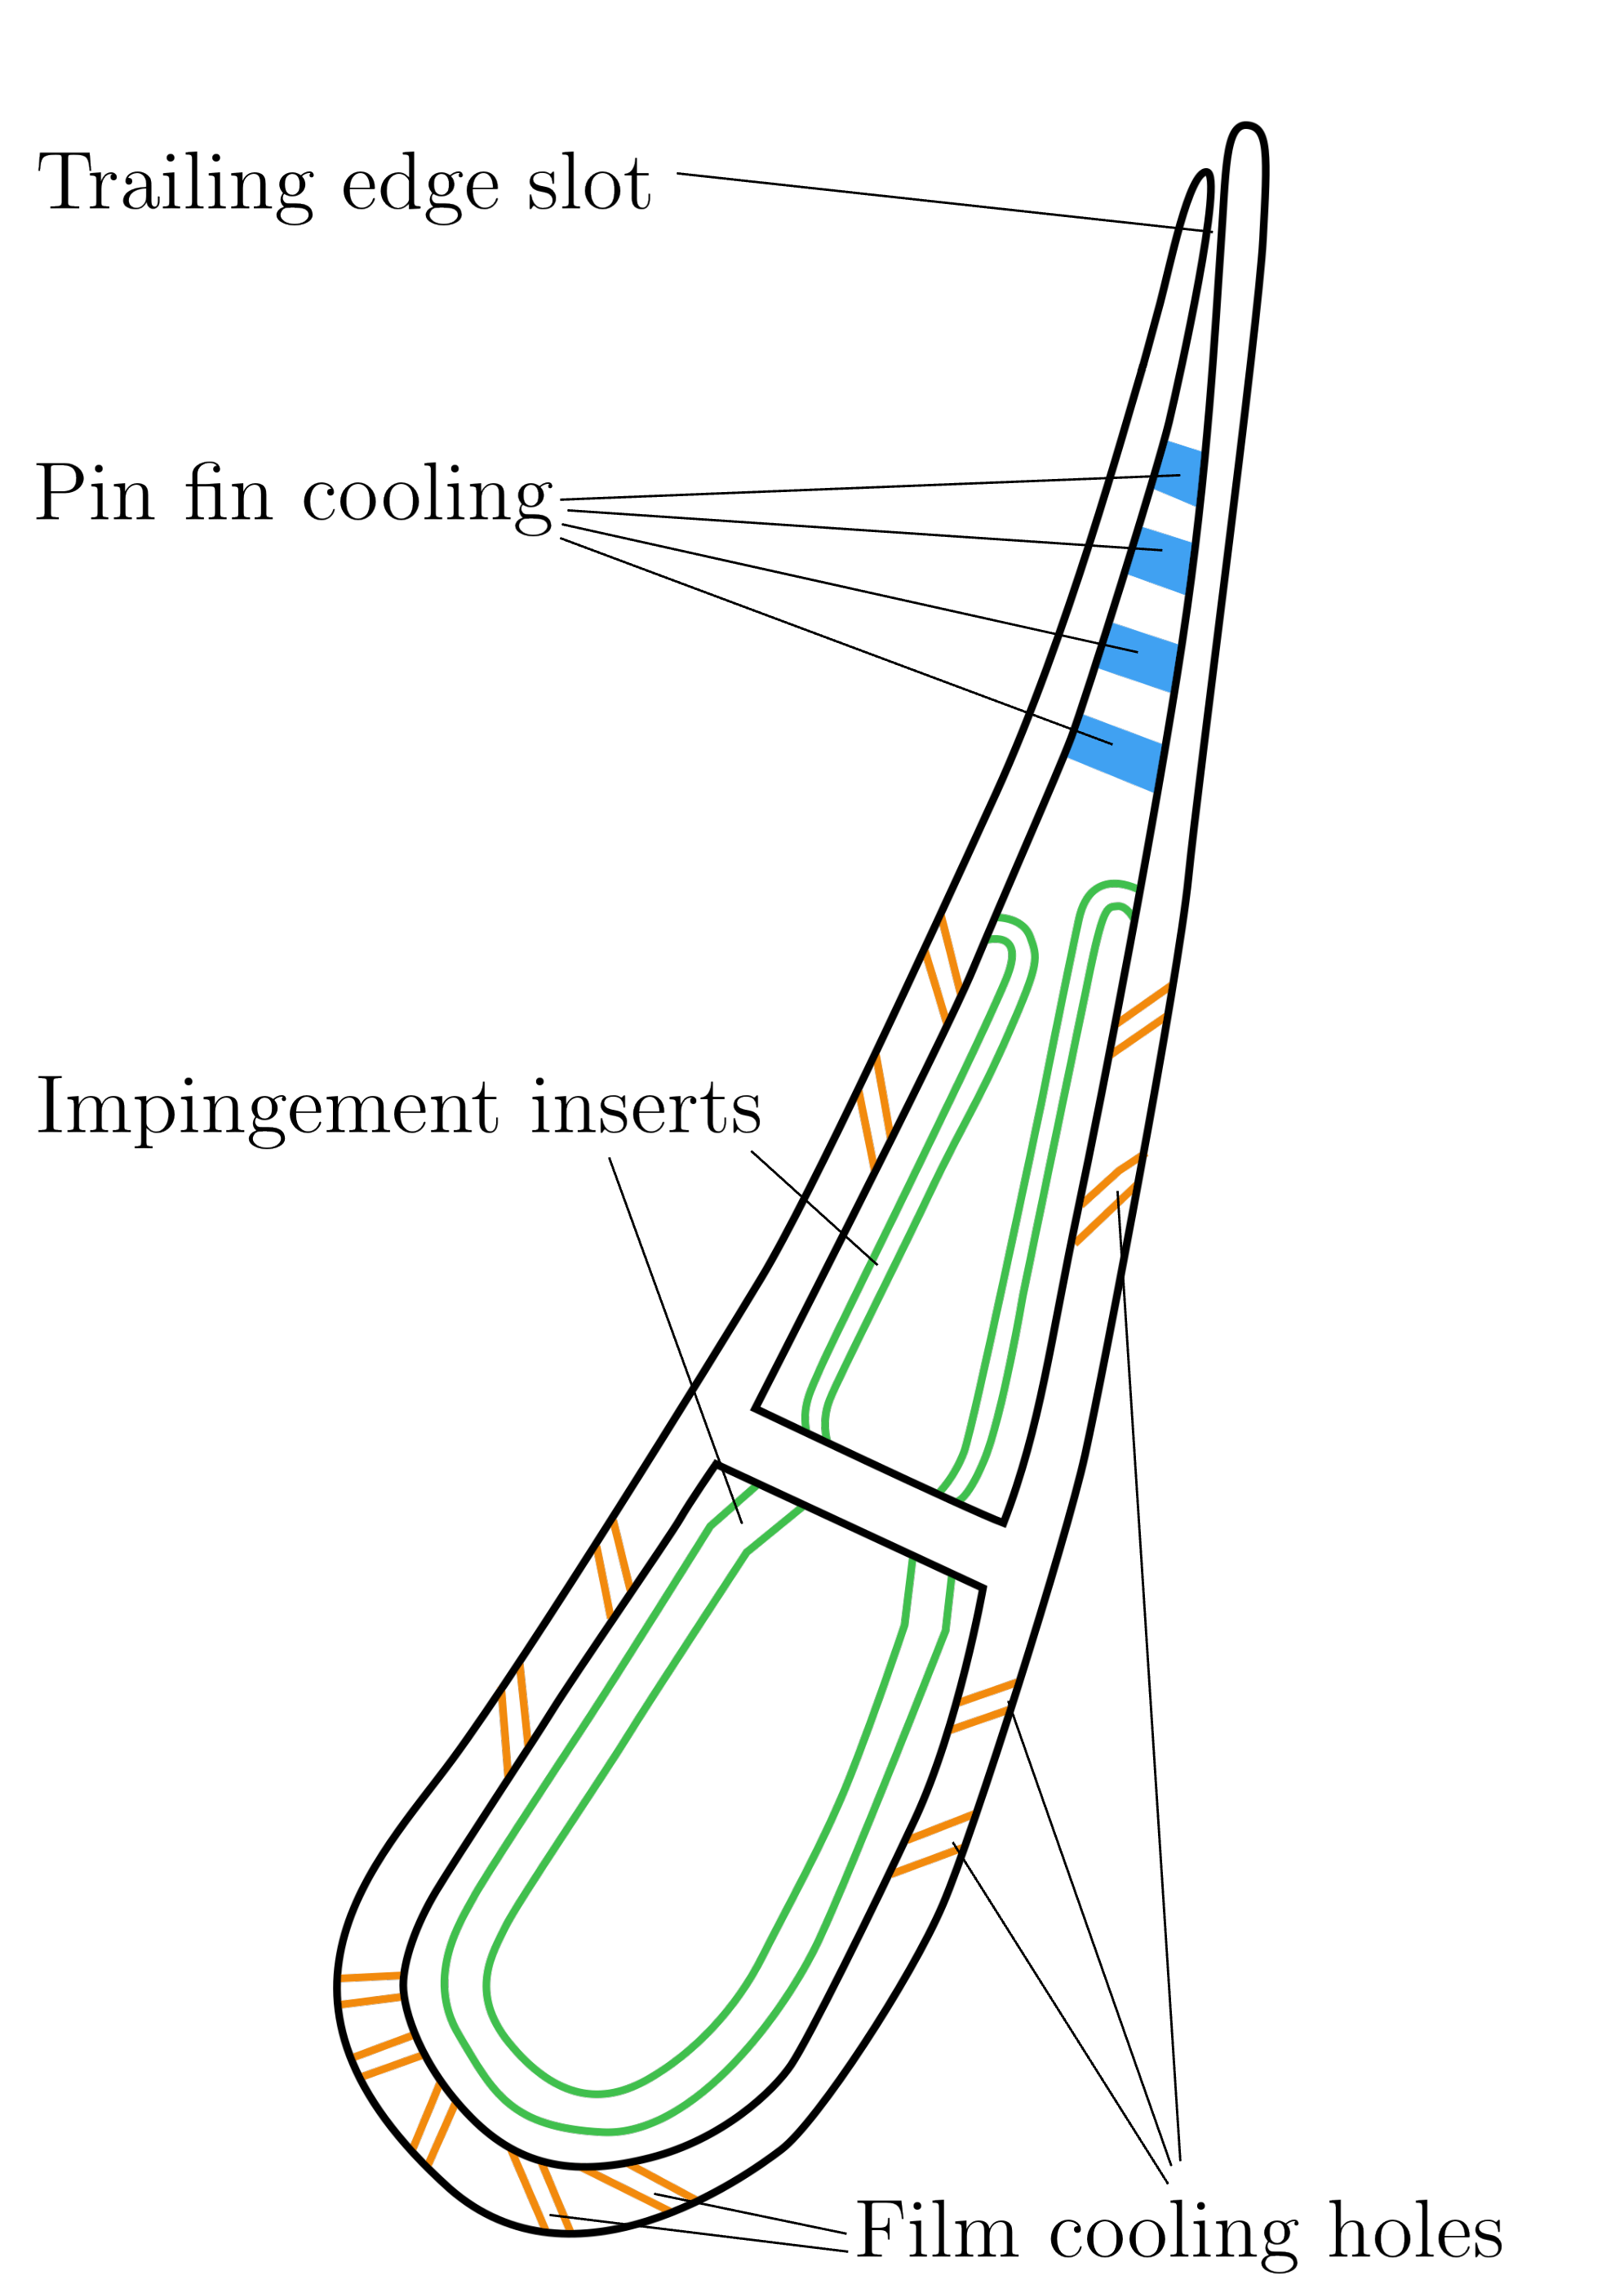
\includegraphics[width=.9\textwidth]{../../assets/gth_rebuild/11.png}
				\caption{Stator im Profil.}
			\end{subfigure}
		\end{figure}
	\end{minipage}
	\vfill
\end{frame}

\begin{frame}
	\frametitle{Problemstellung / Geometrieerzeugung}
	\vspace{-0.5cm}\hspace{-0.5cm}
	\begin{minipage}[t]{0.65\textwidth}
		\vspace{0.2cm}
		Mit CAD-Software lassen sich solche Strukturen erstellen. Leider ist der Prozess zeitaufwendig und schwierig.
		\begin{itemize}
			\item Parametrische Werkzeuge innerhalb herkömmlicher CAD Software bieten meistens nur eine semantische Schnittstelle für einfache Strukturen (z.B. Zylinder, Quader, Kegel), die sich allerdings beliebig miteinander kombinieren lassen (z.B. Verschneiden, Vereinen).
			\item Durch die Erstellung von Freiformkörpern gibt es gar keine parametrische Schnittstelle zur "mechanischen Realität". Dies beeinträchtigt die Möglichkeit zur einfachen Modifikation.
			\item[\textrightarrow] In beiden Fällen entsteht ein Modell, welches schwierig zu erstellen/modifizieren ist.
		\end{itemize}
		\vspace{1em}
		\textbf{Unser Lösungsansatz:} Wir erstellen uns eine eigene CAD-Software, die für uns die speziellen Kühlstrukturen mithilfe von bedeutungsträchtigen Parametern erstellt. Damit geht die Erstellung und Modifikation von Kühlungsgeometrien einfacher und schneller.
	\end{minipage}
	\begin{minipage}[t]{0.35\textwidth}
		\begin{figure}[H]
			\centering
			\begin{subfigure}{0.8\textwidth}
				\centering
				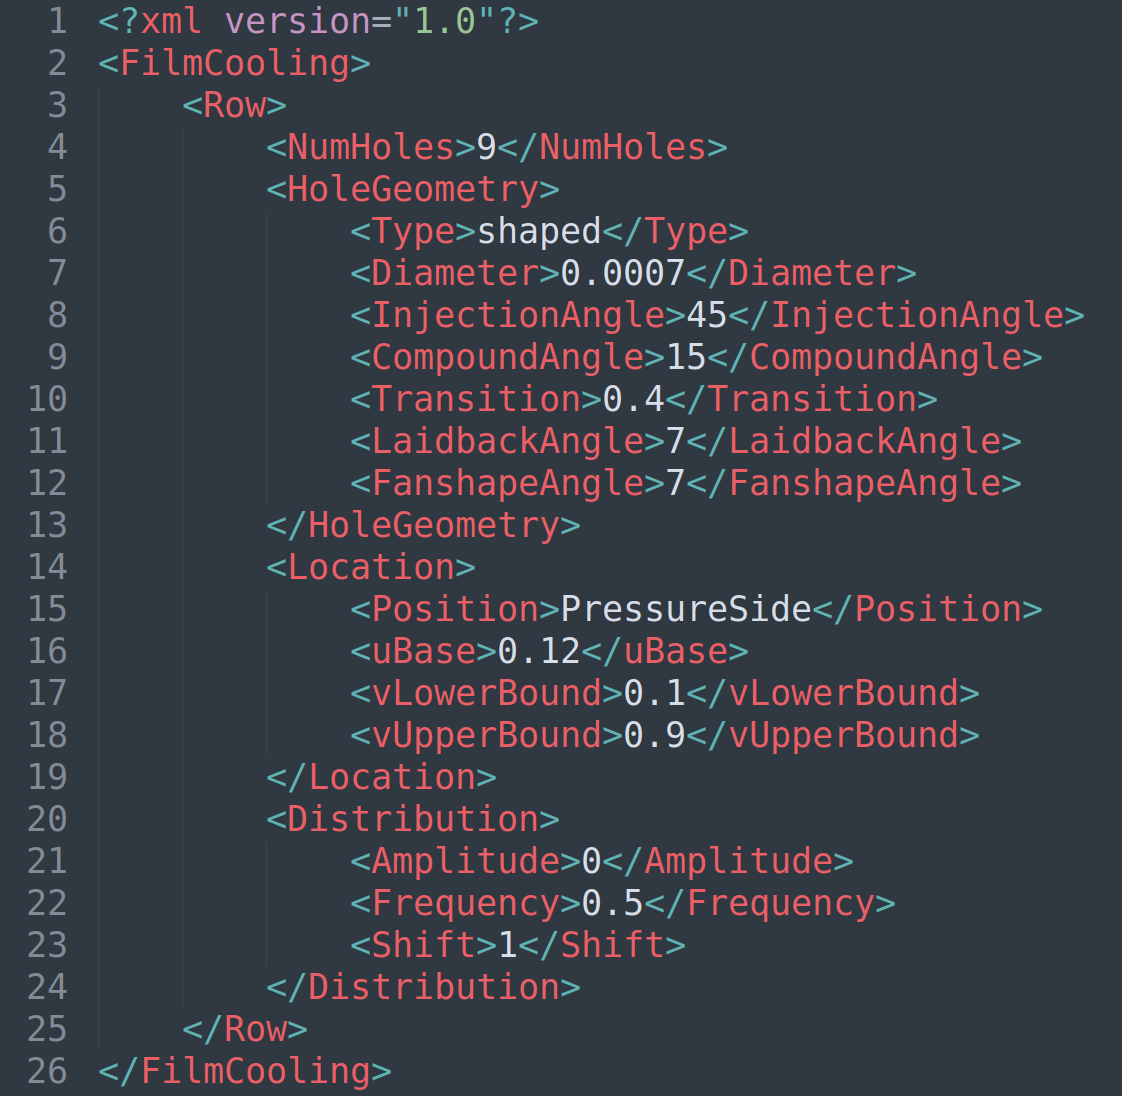
\includegraphics[width=\textwidth]{images/filmxml.png}
			\end{subfigure}\\
			$\Downarrow$\\
			\begin{subfigure}{0.8\textwidth}
				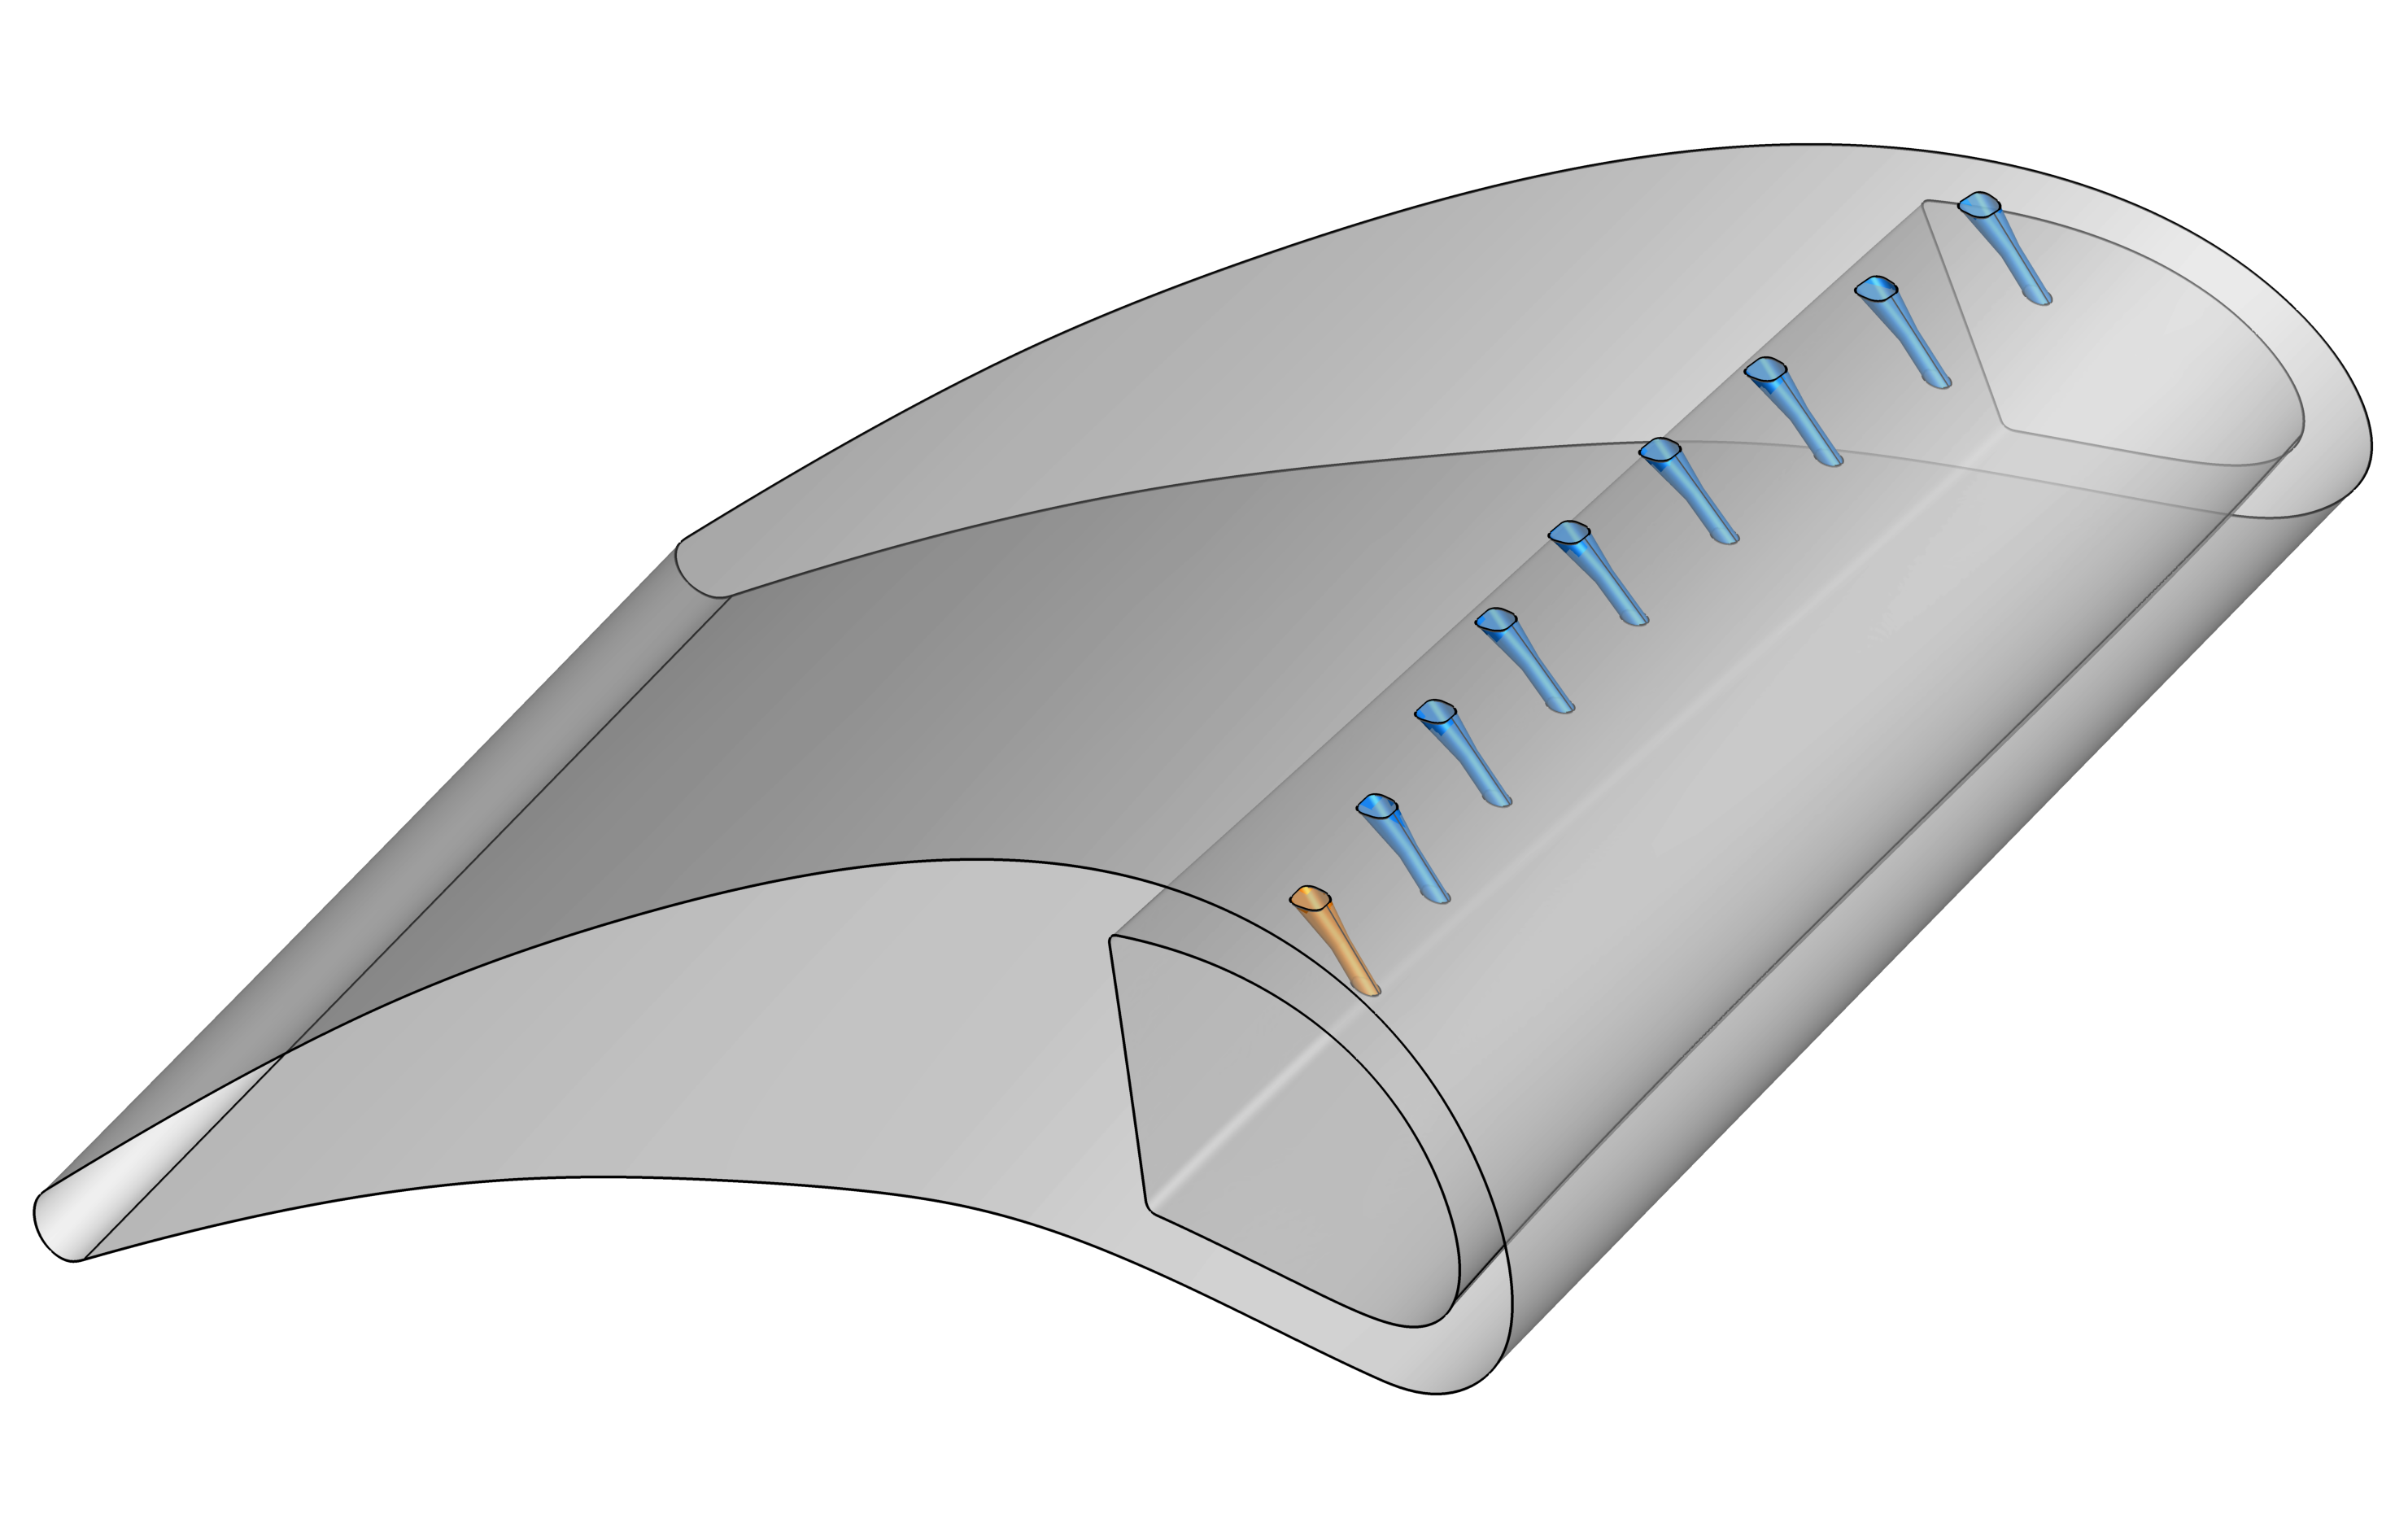
\includegraphics[width=\textwidth]{../../tec/holes/22edit.png}
			\end{subfigure}
		\end{figure}
	\end{minipage}
	\vfill
\end{frame}

\begin{frame}
	\frametitle{Problemstellung / To-Do-Liste}
	\vspace{-0.5cm}\hspace{-0.5cm}
	\begin{minipage}[t]{.8\textwidth}
		Notwendige geometrische Operationen:
		\begin{itemize}
			\item[\ding{108}] 	Implementation von NURBS-Kurven und -Flächen
			\item[\ding{108}]	Projektion von Punkten auf NURBS-Objekte
			\item[\ding{109}]	Offset-Kurven
			\item[\ding{109}]	Schnitt Halbgerade/Kurve in 2D (Ray-Marching)
			\item[\ding{108}]	Schnitt Halbgerade/NURBS-Fläche in 3D
			\item[\ding{108}]	Schnitt Kurve/Kurve
			\item[\ding{108}]	Schnitt Ebene/NURBS-Fläche in 3D
			\item[\ding{109}]	Fillets in 2D
		\end{itemize}
	\end{minipage}
	\vfill
\end{frame}

\end{document}